
\section{Face Recognition}

% \subsection{The EigenFace Approach}
% Much of the previous work on automated face recognition has ignored the issue of just what aspects of the face stimulus are important for identification.
% This suggested that an information theory approach of encoding and decoding face images may give insight into the information content of face images, emphasizing the significant local and global features. Such features may or may not be directly related to our intuitive notion of face features such as the eyes, nose, lips, and hair. \\
% In the language of information theory, the relevant information in a face image should be extracted, encode it as efficiently as possible, and compare one face encoding with a database of models encoded similarly. \\
% A simple approach to extracting the information contained in an image of a face is to somehow capture the variation in a collection of face images, independent of any judgment of features, and use this information to encode and compare individual face images. \\
% In mathematical terms, we wish to find the principal components of the distribution of faces, or the eigenvectors of the covariance matrix of the set of face images, treating an image as a vector in a very high dimensional space. The eigenvectors are ordered, each one accounting for a different amount of the variation among the face images. \\
% These eigenvectors can be thought of as a set of features that together characterize the variation between face images. Each image location contributes more or less to each eigenvector, so that the eigenvector is displayed as a sort of ghostly face, which is called an eigenface (see Figure \ref{fig:meigenface}). \\
% The approach to face recognition using the eigenface approach involves the
% following initiation operations: \\
% \begin{enumerate}
%   \item Acquire an initial set of characteristic face images (the training set). \\
%         This set should include a number of images for each person, with some
%         variation in expression and in the lighting. \\
%         (say \textbf{4} images of \textbf{10} people, so \textbf{M = 40}.)
%   \item Calculate the eigenfaces from the training set, keeping only the M images that correspond to the highest eigenvalues. \\
%         These M images define the \textit{face space}. As new faces are experienced, the eigenfaces can be updated or re-calculated.
%         \begin{enumerate}
%           \item Calculate the (M x M) matrix L, find it's eigenvectors and eigenvalues, and choose the M' eigenvectors with the highest associated eigenvalues. \\
%                 (Let $ M' = 10 $ in this example.)
%           \item Combine the normalized training set of images (according to
%                 equation (\ref{eq:six})) to produce the (say, $ M' = 10 $) eigenfaces $ u_{k} $. \\
%                 \begin{equation} \label{eq:six}
%                   u_{l} = \sum_{k = 1}^{M} v_{lk}\Phi_{k} \hspace{10 mm}, l = 1,2,\ldots,M
%                 \end{equation}
%           \item For each known individual, calculate the class vector $ \Omega_{k} $ by averaging the eigenface pattern vectors $ \Omega $ (from equation (\ref{eq:eight})) calculated from the original images (four, in this example) of the individual. \\
%                 \begin{equation} \label{eq:eight}
%                   \epsilon_{k}^{2} = || (\Omega - \Omega_{k}) ||^{2}
%                 \end{equation}
%                 Choose a threshold $ \theta_{\epsilon} $ that defines the maximum allowable distance from any face class, and a threshold $ \theta_{\epsilon} $ that defines the maximum allowable distance from face space.
%                 (according to equation (\ref{eq:nine})) \\
%                 \begin{equation} \label{eq:nine}
%                   \epsilon^{2} = || (\Phi - \Phi_{f}) ||^{2}
%                 \end{equation}
%           \item For each new face image to be identified, calculate it's pattern
%                 vector $ \Omega $, the distance $ \epsilon_{i} $ to each known
%                 class, and the distance $ \epsilon $ to face space. \\
%                 If the minimum distance $ \epsilon_{k} < \Theta_{\epsilon} $
%                 and the distance $ \epsilon < \Theta_{\epsilon} $, classify the
%                 input face as the individual associated with the class vector
%                 $ \Omega_{k} $. \\
%                 If the minimum distance $ \epsilon_{k} > \Theta_{\epsilon} $ but
%                 distance $ \epsilon < \Theta_{\epsilon} $, Then the image may be
%                 classified as unknown, and optionally used to begin a new face class.
%         \end{enumerate}
%   \item If the new image is classified as a known individual, this image may be added
%         to the original set of familiar face images, and the eigenfaces may be recalculated
%         (steps 1-2). This gives the opportunity to modify the face space as the
%         system encounters more instances of known faces.
%   \item Calculate the corresponding in M-dimensional weight space for each known
%         individual, by projecting the face images onto the face space.
% \end{enumerate}
% The above initialization operations can be performed from time to time whenever
% there is free excess computational capacity, available in the system. \\
% Having initialized the system, the following steps are then used to recognize
% new face images: \\
% \begin{enumerate}
%   \item Calculate a set of weights based on the input image and the M eigenfaces
%         by projecting the input image onto each of the eigenfaces.
%   \item Determine if the image is a face (whether known or unknown) by checking
%         to see if the image is sufficiently close to face space.
%   \item If it is a face, classify the weight pattern as either a known person or
%         as unknown.
%   \item Update the eigenfaces and/or weight pattern.
%   \item If the same unknown face is seen several times, calculate its characteristic
%         weight pattern and incorporate into the known faces.
% \end{enumerate}
%
% \begin{figure}[!t]
% \centering
% 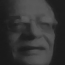
\includegraphics[width=1.5in]{./gulzar.png}
% % where an .eps filename suffix will be assumed under latex,
% % and a .pdf suffix will be assumed for pdflatex; or what has been declared
% % via \DeclareGraphicsExtensions.
% \caption{Mean Eigen Face}
% \label{fig:meigenface}
% \end{figure}
%
% In the prototype implemented using the eigenfaces approach, calculation of the
% eigenfaces is done as part of the training process. \\
% The recognition, using the eigenfaces approach, takes about 90 seconds
% implemented in Python on an Intel Core i5, using face images of size 132 x 132. \\

\subsection{The Local Binary Pattern Histogram Approach}
% It is observed that if the above program is run without any alterations, trained with a specific person, and another untrained face is introduced, then it will be recognized as the trained person. \\
The methods to improve the accuracy of the Face Recognizer have been made more stringent. The threshold used to control unknown faces, in the case of the EigenFaceRecognizer, from the calculated distance can be adjusted to allow better accuracy. \\

\subsection{Principle Component Analysis}

The EigenFaceRecognizer class applies PCA on each image, the results of which will be an array of Eigen values that a neural network can be trained to recognize. \\
The LBPHFaceRecognizer uses Local Binary Patterns (LBP) to create a feature vector using a Support Vector Machine or some other machine learning algorithm. \\

\subsection{The Local Binary Pattern Histogram Classifier}
The LBPH recognizer takes five variables: \\
\begin{description}
  \item[\textbf{radius}] \quad
  The radius used for building the Circular Local Binary Pattern.

  \item[\textbf{neighbors}] \quad
  The number of sample points to build a Circular Local Binary Pattern from.
  OpenCV documentation suggests the value eight sample points.
  The more the number of sample points, higher will be the computational cost.

  \item[\textbf{grid\_x}] \quad
  The number of cells in the horizontal direction.
  The common value used in publications is eight.
  The more cells, the finer the grid, the higher the dimensionality of the resulting feature vector.

  \item[\textbf{grid\_y}] \quad
  The number of cells in the vertical direction.
  The common value used in publications is eight.
  The more cells, the finer the grid, the higher the dimensionality of the resulting feature vector.

  \item[\textbf{threshold}] \quad
  The threshold applied in the prediction.
  If the distance to the nearest neighbor is larger than the threshold, the method returns \textbf{-1}.
\end{description}

\begin{figure}[!t]
\centering
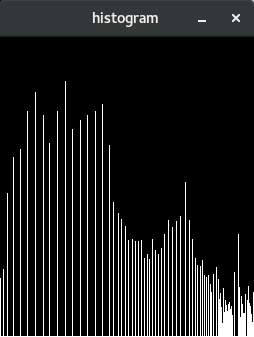
\includegraphics[width=1.5in]{./histogram.png}
% where an .eps filename suffix will be assumed under latex,
% and a .pdf suffix will be assumed for pdflatex; or what has been declared
% via \DeclareGraphicsExtensions.
\caption{Local Binary Pattern}
\label{fig:lbph}
\end{figure}

In the prototype implemented using the LBPH Approach (see Figure (\ref{fig:lbph})), calculation of the
LBP is done as part of the training process. \\
The recognition, using the LBPH approach, takes about 30 milliseconds
implemented in Python on an Intel Core i5, using face images of size 132 x 132. \\
